\section{Analytical Investigation}

\begin{center}
	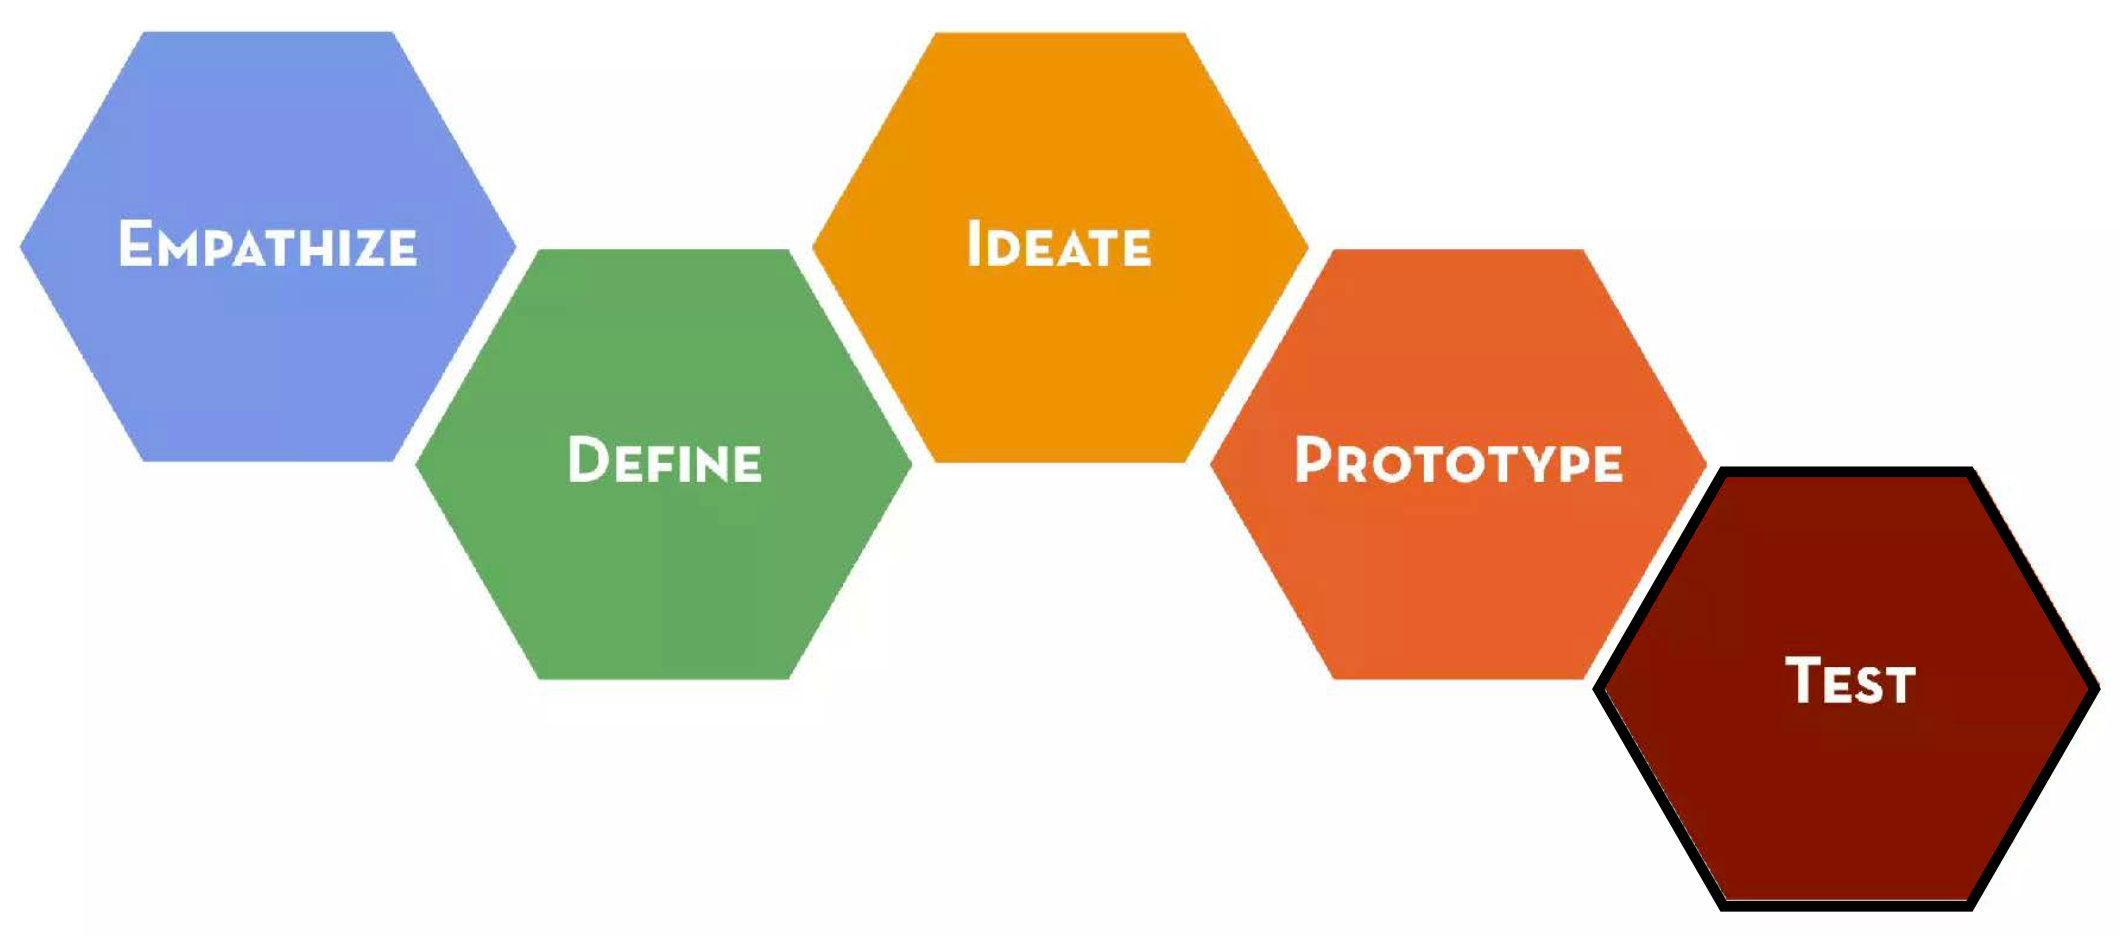
\includegraphics[width=\linewidth]{test.png}
\end{center}

Is performed by usability experts and domain experts. They use their knowledge of users and technology to assess the usability and user experience. Result can be formal or informal reports. 

Two types of analytical investigation: 

\begin{enumerate}
    \item Usability and UX inspection (Design, cognitive walktrhoughs, heuristic evaluation)
    \item Predictive user performance models (GOMS, KLM)
\end{enumerate}

\medskip

\textbf{1. Usability and UX inspection} \smallskip

\textit{Cognitive Walkthroughs} \smallskip

Evaluate design by experts, with the goal of exploring the design on behalf of the users.
Difference to UX inspection: Ux inspection only one aspect of a design presented to experts. Cognitive walkthrough: More focussed on ease-of-learning.  \medskip

\textit{Heuristic Evaluation} \smallskip

Heuristics are design guidelines. 
Examine the interface, judge is compliance with recognized usability principles (heuristics).
Is cheap, fast and easy to use. Is developed for inexperiences practicioners, experts can be limited through heuristics. Can be done on paper-only prototypes. \smallskip


\begin{enumerate}
    \item Briefing to tell evaluators what to do
    \item Each evaluator inspects interface alone (at least twice, get feel for flow of interaction and scope of system, also focus on specific interface elements)
    \item evaluators aggregate findings
    \item debriefing session, discussion of possible redesigns for major UX problems, look as positive aspects
\end{enumerate}

Optimally between 3 and 5 evaluators. Limited because it does not encourage to take a rich and comprehensive view of interaction. Its only a rough outline, and expert find problems withs inspection not heuristics. 
Danger of overestimating heuristics and use for any evaluation. \medskip

\textbf{Nielsen's Heuristics} \smallskip


\textit{1. Visibility of system status} \smallskip

System should always keep users informed about what is going on, through approp. feedback in reasonable time. \medskip

\textit{2. Match between system and the real world} \smallskip

System should speak the users' language, wih words, phrases and concepts familiar to the user, rathen thans system-oriented terms. Follow real world conventions, make info appear in natural and logical order. \medskip

\textit{3. User control and freedom} \smallskip

Users need a clearly marked emergency exit from unwanted state, if chosen system functions by mistake. \medskip

\textit{4. Consistency and standards} \smallskip

User should not have to wonder whether different words, situations or actions mean the same thing. \medskip

\textit{5. Error prevention} \smallskip

Good error messages, but better is design that prevents a proble  from occurring in the first place. Eliminate error-prone conditions or check for them and give users a confirmation option before commiting to the action. \medskip

\textit{6. Recognition rather than recall} \smallskip

Minimize the user's memory load by making opjects, options and actions visible. Instructions for use of the system should be visible or easily retrievable, whenever appropriate. \medskip

\textit{7. Flexibility and efficiency of use} \smallskip

Accelerators may often speed up the interaction for the expert user, such that the system can support both inexperienced and experienced users. \medskip

\textit{8. Asthetic ans minimalist design} \smallskip

Dialogs should not contain irrelevant or rarely needed information. Extra infos compete with the relevant units of information. \medskip


\textit{9. Help users recognize, diagnose and recover from errors} \smallskip

Error messages should be expressed in plain language, precisely indicate the problem and constructively suggest a solution.

\textit{10. Help and documentation} \smallskip

Even it is better if the system can be used without documentation, it may be necessary to provide help and documentation. Should be easy to reach, list concrete steps and should not be too extensive. \medskip


\textbf{2. Predictive User performance models} \smallskip

Way of evaluating roducts or design without directly involving users. Estimated of efficiency of systems for different tasks. \smallskip

We use GOMS to model knowledge about the system and cognitive provesses involved when users interact with systems. 

We use KLM to provide numerical predictions to performance and estimate chains of operations. \medskip

\textbf{GOMS model} \smallskip

\textit{Goals} \smallskip

The state the user wants to achieve. \medskip

\textit{Operators} \smallskip

Cognitive processes and pyhsical actions needed to attain the coals (mouse click etc.) \medskip

\textit{Methods} \smallskip

Procedures for accomplishing th goals, drage mouse over search gield, type in term, press go etc ... \medskip

\textit{Selection Rules} \smallskip

Decide which method to select when there is more than one. \smallskip

Goms example:
\begin{center}
	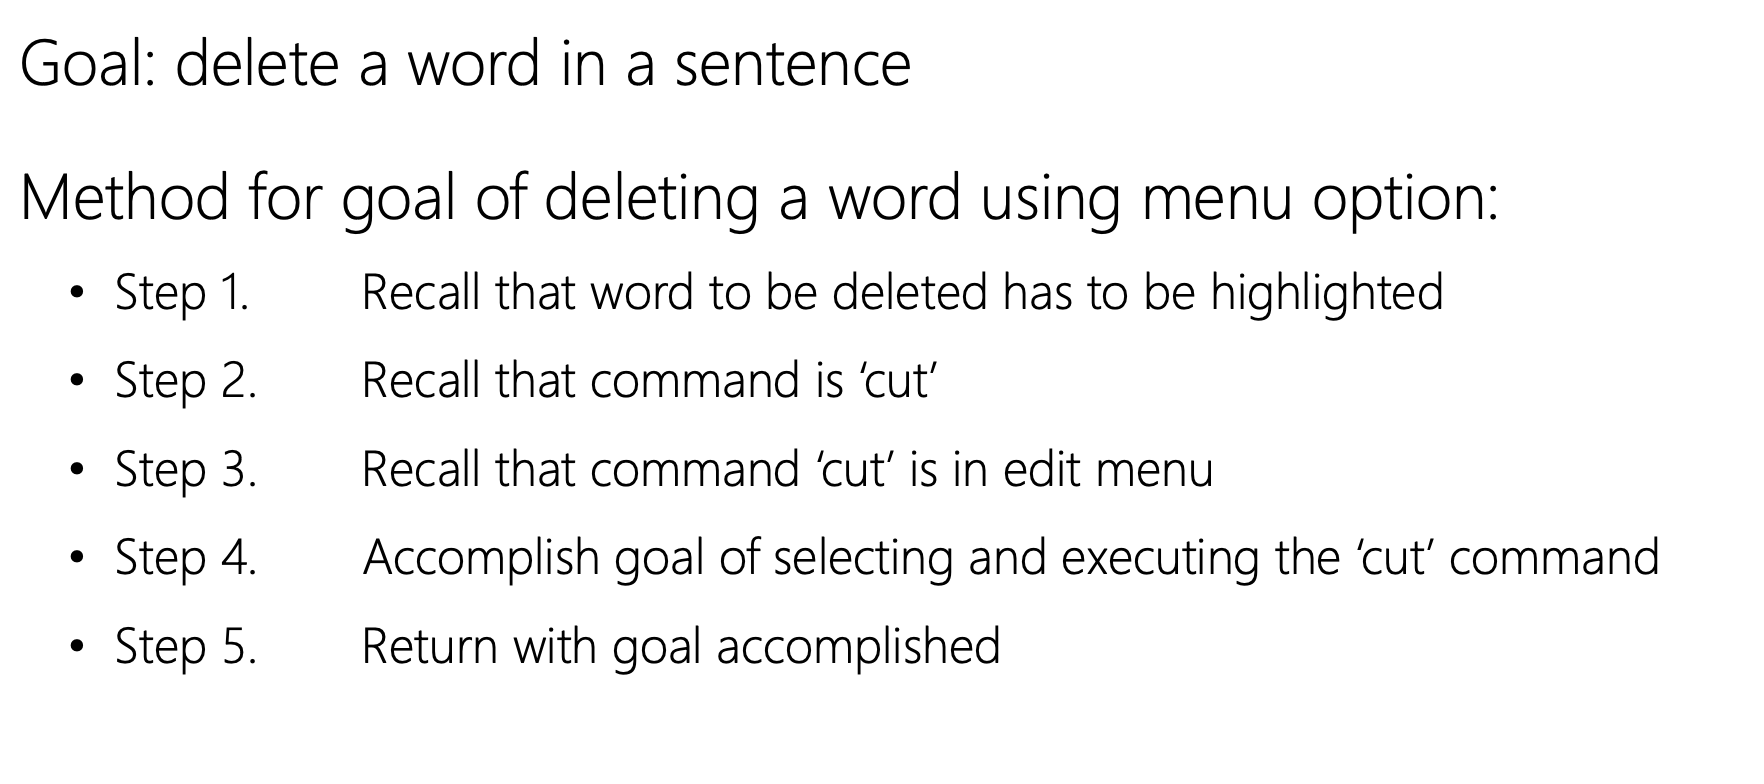
\includegraphics[width=\linewidth]{goms_example.png}
\end{center}

\textbf{Keystroke Level model (KLM)} \smallskip

Mesarues and compares execution times. 

\begin{center}
	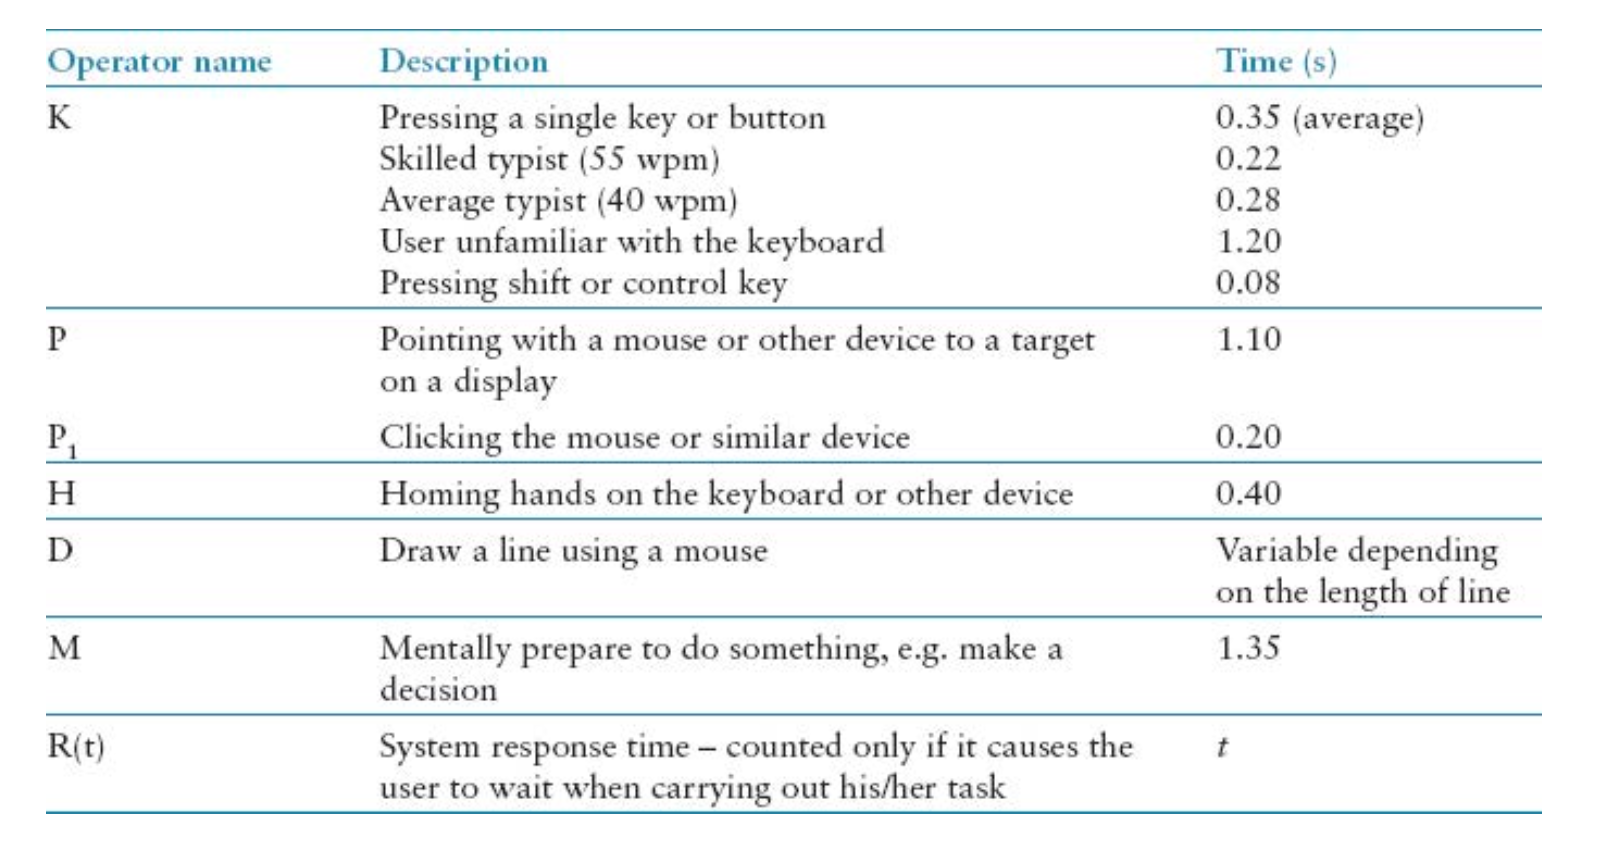
\includegraphics[width=\linewidth]{klm_model.png}
\end{center}


\textit{Predictive models strengths and weaknesses} \medskip


\begin{itemize}
    \item Relatively to perform comaprative analysis for different interfaces and prototypes, specifications. 
    \item Can only model high-level tasks, involving small set of high routine low level tasks
    \item Only valid for predictable/expert behavior (no multi-tasking, fatigue, learning effects etc)
\end{itemize}



